\documentclass[conference]{IEEEtran}

\usepackage[utf8]{inputenc}
\usepackage[T1]{fontenc}
\usepackage{amsmath,amssymb}
\usepackage{graphicx}
\usepackage{booktabs}
\usepackage{url}
\usepackage{hyperref}
\usepackage{xcolor}
\usepackage{tikz}
\usetikzlibrary{arrows.meta,positioning,shapes.geometric,fit}
\usepackage{multirow}
\usepackage{enumitem}

\hypersetup{colorlinks=true, linkcolor=black, citecolor=black, urlcolor=blue}

\IEEEoverridecommandlockouts
\begin{document}

\title{Muscle Memory for Machines: Cognitive Motor\\Learning for Autonomous Desktop Agents}

\author{
\IEEEauthorblockN{Victor Santiago Monta\~{n}o Diaz\thanks{Source code: \url{https://github.com/santiagomd11/Agent-Forge}}}
\IEEEauthorblockA{Independent Researcher}
}

\maketitle

% ============================================================
% ABSTRACT
% ============================================================
\begin{abstract}
Current AI computer use agents treat every click as a first-time click. No matter how many times an agent clicks the same button, the movement takes the same amount of time. Humans, by contrast, get faster with practice. We present a cross-platform computer use system, exposed as a Model Context Protocol (MCP) server, whose key innovation is a spatiotemporal motor memory cache that lets any MCP-compatible AI agent develop ``muscle memory.'' The cache combines eight mechanisms: R-Tree spatial indexing, Power Law of Practice speed-up, Fitts's Law movement timing, WindMouse trajectory adaptation, temporal decay, EMA position smoothing, action sequence prediction, and cross-session persistence. A three-layer resolution hierarchy ensures that \emph{every} mouse interaction builds cache entries, regardless of application or platform. The system exposes 20 tools across four platforms (Windows, WSL2, Linux with X11 and Wayland, and macOS) and requires no SDK integration from the host agent. Testing on real desktop applications shows cache hits growing across sessions and across independent agent instances, with movement durations dropping to 30\% of initial values. To our knowledge, this is the first system to apply cognitive science motor learning models to the execution layer of AI GUI agents, deployed as a ready-to-use MCP server.
\end{abstract}

\begin{IEEEkeywords}
computer use agents, Model Context Protocol, muscle memory, motor learning, GUI automation, spatial caching
\end{IEEEkeywords}

% ============================================================
% I. INTRODUCTION
% ============================================================
\section{Introduction}

A human expert's 100th click on ``Save'' is fast and automatic. An AI computer use agent's 100th click on the same button takes exactly as long as its first. Current GUI agents have no concept of motor learning.

Recent large language models (LLMs) have enabled a new class of \emph{computer use agents} (CUAs) that interact with desktop applications through screenshots and mouse/keyboard input~\cite{anthropic2024computer,openai2025operator,zhang2024ufo}. These systems are good at deciding \emph{what} to click based on visual understanding. But the execution layer, \emph{how} the cursor reaches the target, is stateless. Every mouse movement is computed from scratch, even for buttons the agent has clicked hundreds of times before.

Humans work differently. Decades of cognitive science research show that repeated aimed movements follow the \emph{Power Law of Practice}~\cite{newell1981}: movement time decreases as a power function of repetition count. The base timing of aimed movements follows \emph{Fitts's Law}~\cite{fitts1954}, and unused motor memories fade over time following the \emph{Ebbinghaus forgetting curve}~\cite{ebbinghaus1885}.

We present a \emph{spatiotemporal motor memory cache} that brings this behavior to GUI agents. The system sits in the execution layer and works with any LLM backbone. It combines eight mechanisms:

\begin{enumerate}[noitemsep,topsep=0pt]
    \item \textbf{R-Tree spatial indexing} for proximity-based element lookup
    \item \textbf{Power Law of Practice} speed-up ($T(n) = T(1) \cdot n^{-0.4}$)
    \item \textbf{Fitts's Law} base movement timing
    \item \textbf{WindMouse trajectory adaptation} (gravity, wind, velocity)
    \item \textbf{Temporal decay}, \textbf{EMA position smoothing}, \textbf{sequence prediction}, and \textbf{cross-session persistence}
\end{enumerate}

A three-layer resolution hierarchy ensures every click is captured: model-provided semantic hints (Layer~3), accessibility API auto-detection (Layer~2), and percentage-bucketed window-relative coordinates (Layer~1). Layer~1 requires only the foreground window's bounding rectangle, so \emph{every} click builds muscle memory, even without accessibility support.

The motor memory cache is one component of a complete computer use system exposed as a Model Context Protocol (MCP)~\cite{mcp2024} server. MCP is an open standard that lets any compatible LLM client (Claude Code, Cursor, custom applications) connect to tool servers without SDK integration. Our server exposes 20~tools covering input (click, type, scroll, drag), perception (screenshots, element detection), and learned navigation (cached path traversal, action templates). The host agent calls \texttt{click(x, y, element\_hint="Save")} and the cache silently accelerates repeated interactions. The system is the execution module of Agent Forge, a meta-framework for creating and running agentic workflows. This paper focuses on the motor memory innovation; the full system architecture is described in Section~III.

% ============================================================
% II. BACKGROUND AND RELATED WORK
% ============================================================
\section{Background and Related Work}

\subsection{Cognitive Science Foundations}

\textbf{Power Law of Practice.} Newell and Rosenbloom~\cite{newell1981} established that the time to perform a task decreases as a power function of the number of practice trials: $T(n) = T(1) \cdot n^{-\alpha}$, where $\alpha$ typically ranges from 0.2 to 0.6 for motor tasks. This law has been observed across diverse domains including cigar rolling, card sorting, and typing.

\textbf{Fitts's Law.} Fitts~\cite{fitts1954} showed that the time required for an aimed movement is logarithmically related to the ratio of distance to target width: $MT = a + b \cdot \log_2(D/W + 1)$. This remains the fundamental model of aimed movements in HCI~\cite{mackenzie1992,soukoreff2004}.

\textbf{Ebbinghaus Forgetting Curve.} Ebbinghaus~\cite{ebbinghaus1885} demonstrated that memory strength decays exponentially with time. We implement this as a half-life model where cache entry confidence halves every 7~days.

\textbf{Motor Memory Consolidation.} Willingham~\cite{willingham1998} described how procedural motor memories become automatic with repetition, moving from explicit to implicit processing. Our system models this through the WindMouse parameter adaptation: as hit count grows, cursor trajectories become straighter and faster, matching the shift from deliberate to automatic motor control.

\subsection{AI GUI Agent Systems}

Current computer use agents do not remember prior interactions at the motor level. Anthropic's Claude Computer Use~\cite{anthropic2024computer} processes screenshots and outputs click coordinates, computing each position from scratch via LLM inference. OpenAI's Operator~\cite{openai2025operator} uses a similar approach. Microsoft's UFO~\cite{zhang2024ufo} adds multi-agent coordination; its successor UFO2 introduced session-based task memory, but neither version addresses motor-level execution adaptation. WebVoyager~\cite{he2024webvoyager} and SeeAct~\cite{zheng2024seeact} focus on web navigation with no motor adaptation. None of these systems learn from repeated interactions with the same target.

\subsection{Motor Simulation and Caching Approaches}

\textbf{UI-Mem}~\cite{uimem2026} builds a hierarchical experience memory for mobile GUI agents, storing workflows, subtask skills, and failure patterns as parameterized templates. It operates at the task planning level (what sequence of actions to take) and uses online reinforcement learning for policy improvement. It does not address motor execution (how the cursor reaches the target), spatial indexing, or movement adaptation.

Table~\ref{tab:comparison} summarizes the feature comparison. No existing system combines even three of our eight mechanisms.

\begin{table}[t]
\centering
\caption{Feature comparison of motor memory mechanisms. Our system is the first to combine all eight.}
\label{tab:comparison}
\small
\setlength{\tabcolsep}{3pt}
\begin{tabular}{@{}lcccc@{}}
\toprule
\textbf{Feature} & \rotatebox{70}{\textbf{Ours}} & \rotatebox{70}{\textbf{Claude CUA}} & \rotatebox{70}{\textbf{OpenAI CUA}} & \rotatebox{70}{\textbf{UI-Mem}} \\
\midrule
R-Tree spatial index       & \checkmark &   &   &   \\
Power Law adaptation       & \checkmark &   &   &   \\
Fitts's Law timing         & \checkmark &   &   &   \\
WindMouse adaptation       & \checkmark &   &   &   \\
Temporal decay             & \checkmark &   &   &   \\
EMA position smoothing     & \checkmark &   &   &   \\
Sequence prediction        & \checkmark &   &   &   \\
Cross-session persistence  & \checkmark &   &   & $\sim$ \\
\bottomrule
\end{tabular}
\end{table}

% ============================================================
% III. SYSTEM ARCHITECTURE
% ============================================================
\section{System Architecture}

\subsection{Overview}

The system is a standalone MCP server that exposes 20~tools to any MCP-compatible LLM client. It handles perception (screenshots with automatic downscaling for vision model accuracy), input execution (click, type, scroll, drag across four OS backends), UI element detection (accessibility APIs and vision-based grounding), and learned navigation (cached path traversal, reusable action templates). Fig.~\ref{fig:architecture} shows the data flow for mouse actions, where the motor memory cache sits between the LLM's decision (what to click) and the platform executor (how to reach the target). The LLM does not need to know the cache exists.

\begin{figure}[t]
\centering
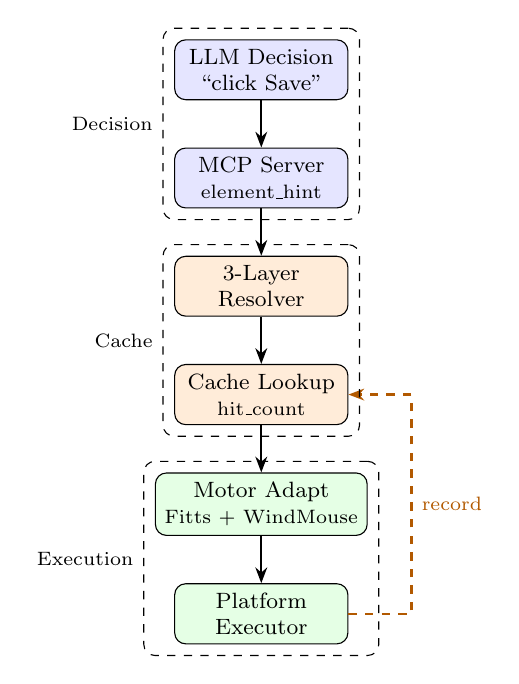
\begin{tikzpicture}[
    node distance=0.6cm,
    box/.style={draw, rounded corners, minimum width=2.2cm, minimum height=0.6cm, font=\footnotesize, align=center},
    layer/.style={draw, dashed, rounded corners, inner sep=4pt, font=\scriptsize\itshape},
    arr/.style={-{Stealth[length=2mm]}, thick},
    >=Stealth
]
    % Decision layer
    \node[box, fill=blue!10] (llm) {LLM Decision\\``click Save''};
    \node[box, below=of llm, fill=blue!10] (mcp) {MCP Server\\{\scriptsize element\_hint}};

    % Cache layer
    \node[box, below=of mcp, fill=orange!15] (resolve) {3-Layer\\Resolver};
    \node[box, below=of resolve, fill=orange!15] (cache) {Cache Lookup\\{\scriptsize hit\_count}};

    % Execution layer
    \node[box, below=of cache, fill=green!10] (adapt) {Motor Adapt\\{\scriptsize Fitts + WindMouse}};
    \node[box, below=of adapt, fill=green!10] (exec) {Platform\\Executor};

    % Arrows
    \draw[arr] (llm) -- (mcp);
    \draw[arr] (mcp) -- (resolve);
    \draw[arr] (resolve) -- (cache);
    \draw[arr] (cache) -- (adapt);
    \draw[arr] (adapt) -- (exec);

    % Cache record arrow (feedback)
    \draw[arr, dashed, color=orange!70!black] (exec.east) -- ++(0.8,0) |- node[right, font=\scriptsize, pos=0.25] {record} (cache.east);

    % Layer labels
    \node[layer, fit=(llm)(mcp), label={[font=\scriptsize]left:Decision}] {};
    \node[layer, fit=(resolve)(cache), label={[font=\scriptsize]left:Cache}] {};
    \node[layer, fit=(adapt)(exec), label={[font=\scriptsize]left:Execution}] {};
\end{tikzpicture}
\caption{Motor memory data flow within the MCP server. The cache mediates between the LLM's decision and the platform executor. A feedback loop records each interaction for future speed-up.}
\label{fig:architecture}
\end{figure}

\subsection{Three-Layer Cache Resolution}

Every mouse action must resolve to a cache key: a combination of \emph{application name} and \emph{element hint}. We use a three-layer hierarchy so that every click is captured:

\textbf{Layer~3 (Model-provided hint).} When the LLM provides a semantic label such as \texttt{element\_hint="Save button"}, this becomes the cache key directly. This is the highest-precision layer but depends on LLM cooperation.

\textbf{Layer~2 (Accessibility API).} When no hint is provided, the engine queries the operating system's accessibility tree for the UI element at the click coordinates, producing keys like \texttt{"button:Save"}. Available for native applications on Windows (UI Automation), Linux (AT-SPI2), and macOS (Accessibility API).

\textbf{Layer~1 (Percentage-bucketed coordinates).} The universal fallback. Requires only the foreground window's bounding rectangle. Click coordinates are converted to window-relative percentages and bucketed at 3\% resolution (${\sim}33$ buckets per axis), producing synthetic hints like \texttt{"@24\%,18\%"}. This layer:

\begin{itemize}[noitemsep,topsep=0pt]
    \item Survives \textbf{window moves} (window-relative coordinates)
    \item Survives \textbf{window resizes} (percentage-based)
    \item Works on \textbf{any application}, including games, Electron apps, and custom UIs with no accessibility support
\end{itemize}

The application name comes from the foreground window's process (e.g., \texttt{"notepad.exe"}, \texttt{"firefox"}). Remote desktop shells (RDP, VNC, terminal emulators) are excluded via a passthrough list because their foreground window is a container, not the actual application being controlled.

\subsection{Three-Tier Cache Lookup}

Given a resolved key \texttt{(app\_name, hint)}, the cache performs a tiered lookup:

\textbf{Tier~1 (Hot cache).} An in-memory Python dictionary keyed by \texttt{"app|hint"} with $O(1)$ exact-match lookup. Sub-microsecond latency. Loaded from SQLite at startup.

\textbf{Tier~2 (R-Tree spatial proximity).} A SQLite R-Tree virtual table~\cite{guttman1984rtree,sqlite_rtree} enables proximity search within a 50-pixel radius, scoped to the same application. Used when Tier~1 misses but coordinates overlap with a known target (e.g., a button that has moved slightly). Latency ${\sim}0.1$ms.

\textbf{Tier~3 (Cache miss).} Returns \texttt{hit\_count=0}. Movement uses default WindMouse parameters.

\subsection{Data Model}

The persistent store uses SQLite with Write-Ahead Logging (WAL) for concurrent read/write safety:

\begin{itemize}[noitemsep,topsep=0pt]
    \item \texttt{memories}: Primary table storing \texttt{app\_name}, \texttt{element\_hint}, EMA-smoothed position $(x, y, w, h)$, \texttt{hit\_count}, \texttt{miss\_count}, timestamps, \texttt{confidence}, and \texttt{prev\_hint} for sequence tracking.
    \item \texttt{memories\_rtree}: R-Tree spatial index on element bounding boxes.
    \item \texttt{sequences}: Action pair tracking (from $\rightarrow$ to) with frequency counts for workflow prediction.
\end{itemize}

An LRU eviction policy caps the cache at 10{,}000 entries, deleting the oldest 10\% by \texttt{last\_hit\_ts} when capacity is reached.

\subsection{Cross-Platform Support}

The system abstracts all platform-specific operations behind a common interface. The cache algorithm itself is platform-agnostic (pure Python, stdlib \texttt{sqlite3}). Backend modules handle cursor control, window queries, and accessibility access:

\begin{itemize}[noitemsep,topsep=0pt]
    \item \textbf{Windows:} Win32 \texttt{SendInput} via ctypes; \texttt{GetForegroundWindow} for window info
    \item \textbf{WSL2:} TCP bridge daemon on Windows (port 19542) relays Win32 calls
    \item \textbf{Linux/X11:} \texttt{xdotool} for window queries; \texttt{/proc/\{pid\}/comm} for process name
    \item \textbf{Linux/Wayland:} Mutter RemoteDesktop DBus interface (\texttt{org.gnome.Mutter.RemoteDesktop}) for pointer and keyboard input; AT-SPI2 accessibility tree for foreground window detection; \texttt{gnome-screenshot} for screen capture
    \item \textbf{macOS:} AppleScript via \texttt{osascript} for window info; \texttt{cliclick} for input
\end{itemize}

Foreground window queries are TTL-cached (50ms in the engine, 100ms on subprocess-based platforms) to amortize overhead.

% ============================================================
% IV. MOTOR ADAPTATION MODEL
% ============================================================
\section{Motor Adaptation Model}

This section details the six mechanisms by which repeated interactions produce faster, more efficient cursor movements.

\subsection{Power Law of Practice}

Following Newell and Rosenbloom~\cite{newell1981}, we model the speed-up of repeated aimed movements as:
\begin{equation}
    T(n) = T_{\text{base}} \cdot n^{-\alpha}, \quad \text{floored at } T_{\text{base}} \cdot \beta
    \label{eq:power_law}
\end{equation}
where $n$ is the hit count (number of prior interactions with the same target), $\alpha = 0.4$ is the learning rate (mid-range for motor tasks), and $\beta = 0.3$ is the asymptotic floor (the target can never be reached faster than 30\% of the initial duration).

Fig.~\ref{fig:power_law} shows the adaptation curve. At $n{=}10$, movement duration has dropped to approximately 40\% of initial. By $n{\approx}20$, it reaches the 30\% floor, modeling the asymptotic performance observed in human motor skill studies.

\begin{figure}[t]
    \centering
    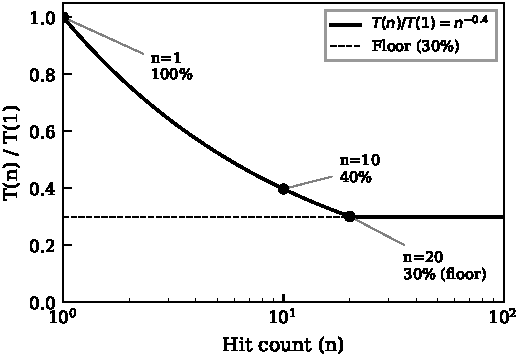
\includegraphics[width=\columnwidth]{figures/fig2_power_law.pdf}
    \caption{Power Law of Practice curve. Movement duration decreases as $n^{-0.4}$ with a 30\% floor. Key points: $n{=}10$ yields ${\sim}40\%$ of initial duration; the floor is reached at $n{\approx}20$. WindMouse parameter adaptation saturates at $n{=}64$.}
    \label{fig:power_law}
\end{figure}

\subsection{Fitts's Law Base Timing}

The initial movement duration $T_{\text{base}}$ is computed using the Shannon formulation of Fitts's Law~\cite{fitts1954,mackenzie1992}:
\begin{equation}
    MT = a + b \cdot \log_2\!\left(\frac{D}{W} + 1\right)
    \label{eq:fitts}
\end{equation}
with $a = 0.05$\,s (base reaction time), $b = 0.11$\,s (movement time coefficient), and a floor of 0.07\,s. Gaussian jitter ($\sigma_a = 0.01$, $\sigma_b = 0.015$) is added to both coefficients to produce human-like variability. The Power Law factor from Eq.~\ref{eq:power_law} is then applied to the resulting duration.

\subsection{WindMouse Trajectory Adaptation}

Cursor trajectories are generated using the WindMouse model, which simulates a particle under two forces: \emph{gravity} (directed toward the target) and \emph{wind} (random perturbation). The model operates in two phases:

\begin{itemize}[noitemsep,topsep=0pt]
    \item \textbf{Ballistic phase} ($d \geq d_h$): Active wind perturbation produces curved, exploratory paths.
    \item \textbf{Homing phase} ($d < d_h$): Wind decays exponentially; gravity dominates, producing precise final approach.
\end{itemize}

where $d$ is the remaining distance and $d_h = 12$\,px is the homing threshold.

As practice count increases, WindMouse parameters adapt via logarithmic scaling (saturating at ${\sim}64$ hits):
\begin{align}
    f &= \min\!\left(1.0,\; \frac{\log_2(n)}{6.0}\right) \label{eq:factor} \\
    G(n) &= 9.0 + 11.0 \cdot f  &&\text{(gravity: 9 $\to$ 20)} \label{eq:gravity} \\
    W(n) &= 3.0 \cdot (1 - 0.7 \cdot f) &&\text{(wind: 3 $\to$ 0.9)} \label{eq:wind} \\
    V(n) &= 20.0 + 15.0 \cdot f &&\text{(max vel: 20 $\to$ 35)} \label{eq:maxvel}
\end{align}

In practice, this means that repeated trajectories become straighter (higher gravity), less wobbly (lower wind), and faster (higher maximum velocity). This matches the transition from deliberate to automatic motor control observed in humans~\cite{willingham1998}. Fig.~\ref{fig:trajectory} illustrates the difference.

\begin{figure}[t]
    \centering
    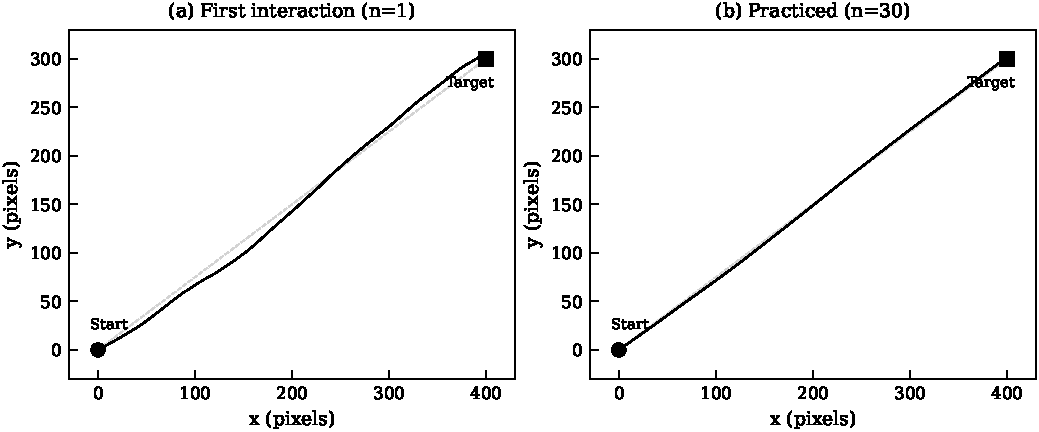
\includegraphics[width=\columnwidth]{figures/fig3_trajectory.pdf}
    \caption{WindMouse cursor trajectories. (a)~First interaction ($n{=}1$): wobbly, exploratory path. (b)~After 30 repetitions: nearly straight, confident path. Both share the same start and end points.}
    \label{fig:trajectory}
\end{figure}

\subsection{Temporal Decay}

Cache entries lose confidence over time, modeling the Ebbinghaus forgetting curve~\cite{ebbinghaus1885}:
\begin{equation}
    c(t) = c_0 \cdot 2^{-t / \tau}
    \label{eq:decay}
\end{equation}
where $\tau = 604{,}800$\,s (7~days) is the half-life. Entries with $c(t) < 0.1$ are treated as forgotten (cache miss). Each successful interaction resets $c_0 = 1.0$. Additionally, each \emph{miss} (target not found where expected) penalizes confidence by $-0.3$, providing rapid adaptation when UI layouts change.

\subsection{EMA Position Smoothing}

UI elements may drift between sessions due to window resizing, layout changes, or dynamic content. We track element positions using an Exponential Moving Average:
\begin{equation}
    \hat{x}_{n+1} = \hat{x}_n + \alpha \cdot (x_{\text{obs}} - \hat{x}_n)
    \label{eq:ema}
\end{equation}
with $\alpha = 0.3$. This smoothing absorbs drift while preserving the learned position of stable elements. The same EMA is applied to element width and height.

\subsection{Sequence Prediction}

The system tracks action transitions as ordered pairs: when the user clicks target $B$ after target $A$, the pair $(A \to B)$ is recorded with a frequency count. The \texttt{predict\_next(app, current\_hint)} function returns the most frequent successor, enabling anticipatory pre-computation of the next target's cache entry. Example from live usage: after the sequence ``WhatsApp taskbar icon $\to$ Andr\'{e}s P Scale chat'' occurs twice, the system predicts this transition with high confidence.

% ============================================================
% V. IMPLEMENTATION
% ============================================================
\section{Implementation}

The system is implemented in Python with zero external dependencies for the core cache (\texttt{sqlite3} is part of the standard library). Key implementation details:

\textbf{Storage.} SQLite with Write-Ahead Logging (WAL) mode and \texttt{NORMAL} synchronous setting balances durability and performance. The R-Tree virtual table is compiled into SQLite by default on all major platforms.

\textbf{MCP server.} The entire system is packaged as an MCP~\cite{mcp2024} server exposing 20~tools over stdio or SSE transport. An LLM client connects by pointing its MCP configuration at the server binary; no SDK integration or code changes are required in the host agent. Screenshots are automatically downscaled to a resolution that balances vision model accuracy with coordinate precision (e.g., 1366\,px wide for a 3840\,px display). Mouse action tools accept an optional \texttt{element\_hint} parameter that feeds the motor memory cache; the engine transparently performs cache resolution, lookup, and recording around each action.

\textbf{Navigation acceleration.} Two higher-level mechanisms skip LLM roundtrips entirely. \emph{Navigate-to} performs BFS path-finding through the sequence graph and executes via cached positions (${\sim}55$\,ms). \emph{Action templates} are named multi-step workflows (click, type, key-press, wait) replayed from the database; a 5-step template completes in under 1\,s vs.\ ${\sim}10{-}20$\,s with LLM processing.

\textbf{Resolution resilience.} Cache entries track both window dimensions and screen resolution at recording time. When the screen resolution changes (e.g., switching monitors or DPI settings), cached coordinates are proportionally rescaled. When only the window is resized, entries are used as-is if coordinates remain in bounds, or treated as misses otherwise. This avoids the distortion that proportional rescaling causes on fixed-grid UIs like spreadsheets.

\textbf{Scale.} The implementation comprises approximately 1{,}100 lines for the cache module (including navigation, resolution resilience, and action templates), 820 lines for the engine facade, and 500 lines for MCP server integration. A test suite of 352 unit tests covers cache CRUD, spatial proximity, temporal decay, power law adaptation, sequence tracking, persistence, eviction, three-layer resolution, passthrough exclusion, percentage-bucket alignment, navigation path-finding, resolution rescaling, DPI-aware accessibility, and action template workflows.

% ============================================================
% VI. EVALUATION
% ============================================================
\section{Evaluation}

\subsection{Experimental Setup}

We evaluate the system on two platforms:

\textbf{Windows~11 + WSL2.} 3840$\times$2400 display (DPI~288), engine on WSL2 with a native Windows bridge daemon for input execution. Test applications include WhatsApp Desktop, with a multi-session workflow: open application from taskbar, navigate to contact, send message, close application, reopen, and edit the sent message.

\textbf{Ubuntu Linux (GNOME/Wayland).} 1366$\times$853 display, engine running natively with Mutter RemoteDesktop for input and AT-SPI2 for window detection. 40~end-to-end tests across six applications (Chrome, GNOME Text Editor, Terminal, Nautilus file manager, GNOME Settings, and desktop shell), covering click, double-click, right-click, drag, type, scroll, and keyboard shortcuts.

\subsection{Cache Growth Across Sessions}

Table~\ref{tab:cache_growth} shows cache metrics across three evaluation sessions. Session~1 is a cold start (all misses). Session~2, performed by an \emph{independent agent instance} with no shared context, achieves cache hits on all previously-seen targets. Session~3 introduces a different contact, demonstrating that independent targets accumulate separate hit counts while shared elements (taskbar icon, message input) benefit from combined usage.

\begin{table}[t]
\centering
\caption{Cache growth across three sessions. Session 2 was performed by an independent agent with zero shared context.}
\label{tab:cache_growth}
\small
\begin{tabular}{@{}lccc@{}}
\toprule
\textbf{Metric} & \textbf{Session 1} & \textbf{Session 2} & \textbf{Session 3} \\
\midrule
Total entries      & 7  & 7  & 12 \\
Cache hits         & 0  & 3  & 5  \\
Avg hit\_count     & 1.0 & 1.4 & 1.5 \\
Unique apps        & 3  & 3  & 3  \\
Sequences recorded & 5  & 7  & 9  \\
New targets        & 7  & 0  & 5  \\
\bottomrule
\end{tabular}
\end{table}

On the Linux platform, the 40~end-to-end tests produced 28~unique cache entries across 6~applications (Chrome: 11, Nautilus: 5, GNOME Terminal: 4, GNOME Text Editor: 4, GNOME Settings: 2, GNOME Shell: 2). All entries were correctly keyed by real application name via AT-SPI2 foreground window detection. Elements with 3+ hits (e.g., browser tabs, address bar, back button) were successfully accessed via cached navigation, executing multi-step click sequences without any LLM roundtrips.

\subsection{Movement Duration Adaptation}

Fig.~\ref{fig:duration} shows the theoretical movement duration for a representative target (500\,px distance, 40\,px width) as a function of interaction count. The Power Law reduction from Eq.~\ref{eq:power_law} produces rapid initial improvement that asymptotes at the 30\% floor after approximately 20 interactions.

\begin{figure}[t]
    \centering
    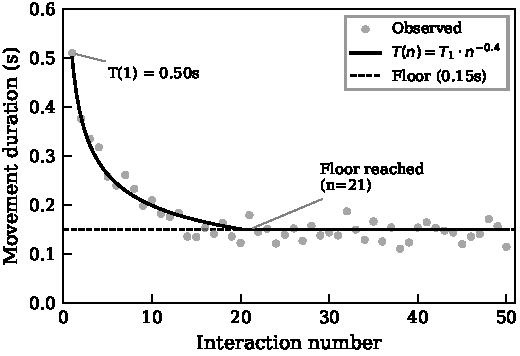
\includegraphics[width=\columnwidth]{figures/fig4_duration.pdf}
    \caption{Simulated movement duration vs.\ interaction count for a representative target (500\,px distance, 40\,px width). Scatter points are sampled from the Power Law model with Gaussian noise ($\sigma{=}0.02$\,s). Duration floors at 30\% of initial value.}
    \label{fig:duration}
\end{figure}

\subsection{Qualitative Observations}

\textbf{Cross-agent persistence.} Agent~B benefits from Agent~A's prior interactions without any explicit knowledge transfer. The shared SQLite database carries the learned positions forward automatically.

\textbf{Resize resilience.} Percentage-based coordinate bucketing (Layer~1) correctly resolves cache hits after window resizing. A target at 25\% of an 800\,px window (200\,px) maps to the same bucket as 25\% of a 1200\,px window (300\,px).

\textbf{Passthrough exclusion.} Remote desktop shells (RDP, VNC) are correctly excluded from caching, so cache entries are not associated with a container application instead of the actual UI being controlled.

\textbf{Wayland compatibility.} On GNOME Wayland, standard tools like \texttt{xdotool} cannot detect the foreground window or inject input. The system uses AT-SPI2 (accessibility tree traversal) for window detection and the Mutter RemoteDesktop DBus interface for absolute pointer positioning. Cache entries are correctly keyed by application name across both X11 and Wayland sessions.

\subsection{Limitations}

The current evaluation has several limitations. First, we have not conducted a formal controlled study comparing movement time and trajectory quality with and without the motor memory cache. Second, the Power Law exponent ($\alpha = 0.4$) and floor ($\beta = 0.3$) are fixed values from the literature rather than fitted to observed agent behavior. Third, the evaluation is single-user on a limited set of applications. Fourth, cursor trajectory ``naturalness'' is inherently subjective without a formal human-likeness metric.

% ============================================================
% VII. DISCUSSION
% ============================================================
\section{Discussion}

\textbf{Works with any LLM.} The cache operates in the execution layer and works with Claude, GPT-4, open-source models, or any other decision framework. It does not change \emph{what} the agent clicks, only how fast the cursor gets there.

\textbf{Trajectories converge naturally.} As hit count grows, the WindMouse parameter adaptation produces trajectories that approach straight lines with smooth velocity profiles. This resembles the minimum-jerk trajectory seen in expert human pointing. We did not program this directly; it emerges from the parameter adaptation.

\textbf{Shared memory across agents.} Because the cache is SQLite on disk, multiple independent agent instances share motor memory automatically. Agent~B moves faster to targets that Agent~A has already used.

\textbf{Living system.} All parameters ($\alpha = 0.4$, $\beta = 0.3$, $\tau = 7$~days, EMA $\alpha = 0.3$, radius = 50~px) are configurable and can be made adaptive as more usage data is collected.

\textbf{Part of a broader framework.} The computer use system is the ``eyes and hands'' module of Agent Forge, a meta-framework for generating agentic workflows through a 7-step orchestrator. Agent Forge alone generates text and code workflows; combined with the computer use server, it targets fully autonomous desktop automation where generated workflows can be executed without human intervention. This integration is ongoing work.

% ============================================================
% VIII. CONCLUSION
% ============================================================
\section{Conclusion and Future Work}

We have presented a cognitive motor learning system for autonomous desktop agents, deployed as a ready-to-use MCP server. Its key contribution is a spatiotemporal motor memory cache grounded in cognitive science (Power Law of Practice, Fitts's Law, Ebbinghaus temporal decay). The three-layer resolution hierarchy and eight adaptation mechanisms let any MCP-compatible agent develop muscle memory that persists across sessions and transfers between agent instances.

Future work includes: (1)~formal A/B studies comparing agent performance with and without the cache; (2)~adaptive $\alpha$ fitting from observed data per element type; (3)~anticipatory cursor movement toward predicted targets before the LLM completes its decision; (4)~a shared cloud cache for fleet-wide motor memory; (5)~integration between the computer use server and Agent Forge's workflow orchestrator for fully autonomous desktop task execution; and (6)~richer accessibility tree information for improved Layer~2 resolution.

% ============================================================
% REFERENCES
% ============================================================
\bibliographystyle{IEEEtran}
\bibliography{references}

\end{document}
